\section{Grundlagen der QM}
\subsection{Schwarzk�rperstrahlung}
\begin{tabular}{p{4cm} p{15cm}}
Schwarzer K�rper	& \begin{itemize}
				\item Ein sK absorbiert elektromagnetische Strahlung vollst�ndig. Somit (wegen Kirchhoffschem Strahlungsgesetz) ist sein Emissionsverm�gen im Vergleich zu beliebigen K�rper maximal ($\epsilon = 1$)
				\item Ein sK l�sst keine Strahlung hindurch und spiegelt oder streut nichts.
				\item Ein beliebiger K�rper kann bei keiner Wellenl�nge mehr Strahlung aussenden als ein sK
                	  \end{itemize}\\
Wiensches Verschiebungsgesetz	& \begin{tabular}[t]{l}
                             	   $\boxed{\lambda_{max} \cdot T = 2.898\cdot 10^{-3} \text{m K}}$\\
				   $[\lambda_{max}] = \mu m$; Wellenl�nge bei der die gr�sste Strahlungsintensit�t auftritt.\\
				   $[T] =$ K; absolute Temperatur der strahlenden Fl�che
				  \end{tabular}\\
Stefan-Boltzmann-Gesetz	& \begin{tabular}[t]{l}
                        	   $\boxed{P = \sigma A \epsilon T^4}$\\
				   $[P] =$ W; Leistung, die auf eine Seite von der Fl�che $A$ abgestrahlt wird.\\
				   $\sigma = 5.67\cdot 10^{-8} \tfrac{W}{m^2K^4}$, Stefan-Boltzmann-Konstante\\
				   $\epsilon \leq 1:$ Emissionsverm�gen
			  \end{tabular}\\
Planck'sches Strahlungsgesetz	& \begin{tabular}[t]{l}
                             	   $\boxed{\rho_E(\nu)d\nu = \frac{8\pi h\nu^3}{c^3}\frac{1}{e^{h\nu/k_B T}-1}d\nu}$\\
				   $\rho_E(\nu)d\nu:$ Volumendichte der thermischen Strahlung in einem Frequenzintervall $[\nu, \nu + \delta\nu]$\\
				   $[\nu] = $s$^{-1}$; Frequenz\\
				   $\rho_E(\lambda)d\lambda = \frac{8\pi hc}{\lambda^5}\frac{1}{e^{hc/\lambda k_B T}-1} d\lambda$
                             	  \end{tabular}\\
\end{tabular}
\subsection{Ebene Welle}
\begin{tabular}{p{4cm} p{7cm} p{8cm}}
Definition		& \multicolumn{2}{l}{$\vec A(\vec r,t) = \operatorname{Re}\left(\vec A_0 e^{ i\left(\vec k\cdot \vec r-\omega t\right)}\right) = \vec A_0 \cos(\vec k\cdot\vec r - \omega t)$}\\
Amplitude		& $\vec A_0$	& Dimension i.A. w�hlbar\\
Wellenvektor		& $\vec k$	&\\
Wellenzahl		& $k = | \vec k | = \frac{2\pi}{\lambda}$	& m$^{-1}$\\
Wellenl�nge		& $\boldsymbol{\lambda = \frac{2\pi}{k}}$	& $m$\\
Kreisfrequenz		& $\omega = 2\pi\nu$ Dispersionsrelation	& s$^{-1}$\\
Frequenz		& $\boldsymbol{\nu = \frac{\omega}{2\pi}}$	& s$^{-1}$\\
Periode			& $T = \frac{1}{\nu} = \frac{2\pi}{\omega}$	& s\\
Phasengeschwindigkeit	& $\boldsymbol{c = \frac{\omega}{k} = \lambda\nu }= \frac{\lambda}{T}$	& m s$^{-1}$\\
Gruppengeschwindigkeit	& $v_G = d\omega / dk$				&  m s$^{-1}$\\
Phase			& $\phi = \vec k \cdot \vec r -\omega t$	& dimensionslos\\
\end{tabular}
\begin{tabular}{p{4cm} p{4cm} p{11cm}}
Abh�ngigkeit von Medium	& \multicolumn{2}{p{15cm}}{Beim �bergang in ein Medium mit Brechungszahl $n = \sqrt{\mu_r \epsilon_r}$ �ndern sich folgende Gr�ssen wie folgt:}\\
			& Frequenz:	& $\nu \rightarrow \nu$\\
			& Wellenl�nge:	& $\lambda \rightarrow \frac{\lambda}{n}$\\
			& Lichtgeschwindigkeit:	& $c \rightarrow \frac{c}{n}$\\
			& Wellenzahl:	& $k \rightarrow k \cdot n$
\end{tabular}
\begin{tabular}{p{4cm} p{15cm}}
Schwebung	& \begin{tabular}[t]{ll}
         	  $E_0 \cdot e^{i(\omega_1 t)} + E_0 \cdot e^{i(\omega_2 t)} = 2E_0 \cos\left( \frac{\Delta\omega}{2} t \right) e^{i\bar{\omega}t}$	& \multirow{3}{*}{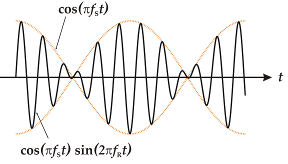
\includegraphics[width = 5cm]{ph_schwebung.png}}\\
		  $\Delta\omega = \omega_1 - \omega_2$\\
		  $\bar{\omega} = \frac{\omega_1 + \omega_2}{2}$
         	  \end{tabular}
		  \\
Beugung		& \begin{tabular}[t]{ll}
		   \multicolumn{2}{l}{$d$ = Breite des Spalts}\\
       		   $d \gg \lambda$	& Keine Beugung\\
		   $d \leq \lambda$	& Welle wird um Spalt gebeugt
       		  \end{tabular}\\
Interferenz	& \begin{tabular}[t]{ll}
           	   Maxima	& $d \sin \theta_m = m\lambda,\quad m = 0,1,2...$\\
		   Minima	& $d \sin \theta_m = (m-\tfrac{1}{2})\lambda,\quad m = 1,2,3,...$\\
		   Intensit�t	& $I = \frac{\sin^2 pz}{\sin^2 z}\quad z = \frac{\pi d}{\lambda}\sin\alpha$ p = \# Spalten
           	  \end{tabular}\\
\end{tabular}
\subsection{Wellenpakete}
Ein Wellenpaket ist eine �berlagerung von ebenen Wellen mit unterschiedlicher Frequenz aber gleicher Phase. Phasengleich bedeutet, dass verschiedene Wellen an einem Punkt $(x,t)$ den gleichen Wert haben.\\
\begin{tabular}{p{9.5cm} |p{9.5cm}}
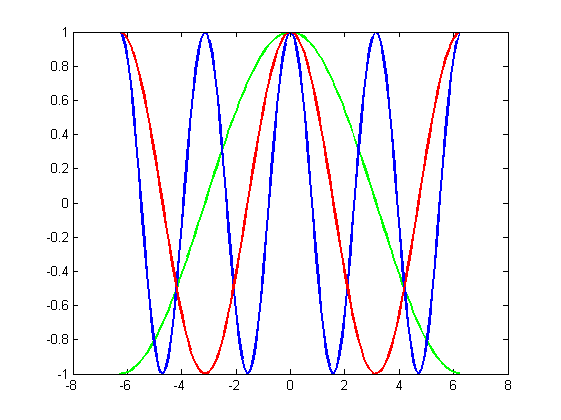
\includegraphics[width = 7cm]{ph_phasengleichewelle.png}	& 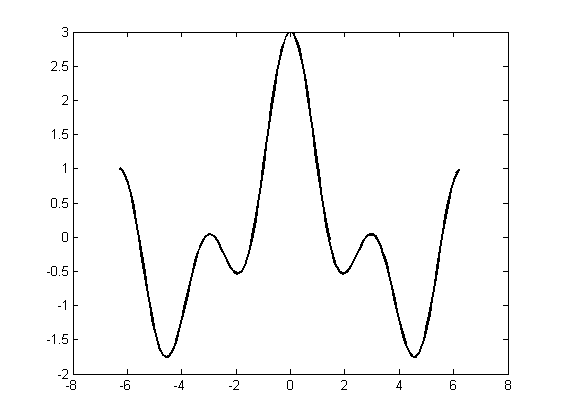
\includegraphics[width = 7cm]{ph_wellenpaket.png}\\
Phasengleiche (um x=0) Cosinusfkt. mit Wellenl�ngen $4\pi$, $2\pi$ und $\pi$	& �berlagerung: $\cos \tfrac{1}{2} x + \cos x + \cos 2x$\\
\end{tabular}\\
\begin{tabular}{p{4cm} p{15cm}}
allgemeinste Lsg. der SG	& $\Psi(x,t) = \sum_n c_n \psi_n(x)e^{-iE_nt/\hbar}\quad\psi_n$ sind L�sungen der SG.\\
Alternative Darstellung		& $\Psi(x,t) = \int g(k)\psi_k(x,t) dk\quad g(k)$ ist eine Gewichtungsfunktion.\\
\multicolumn{2}{p{19cm}}{Der Zusammenhang zwischen einer einzelnen Welle mit bekannter Frequenz und einem Wellenpaket kann auch mittels Fouriertransformation ausgedr�ckt werden:}\\
Welle				& $E(z,t) = F^{-1}\left\lbrace \tilde{E}(z,\omega)\right\rbrace = \frac{1}{2\pi}\int \tilde{E}(z,\omega)e^{i\omega t} d\omega$\\
Frequenzspektrum		& $\tilde{E}(z,\omega) = F\left\lbrace E(z,t) \right\rbrace = \int E(z,t)e^{-i\omega t} dt$\\
FWHM (Full width @ half maximum)	& Sei $f(x_1) = f(x_2) = \frac{1}{2}f(x_\mathrm{max})$ Dann ist FWHM = $|x_1-x_2|$\\
\end{tabular}
\subsubsection{Unterschied Wellenpaket - Welle in Bezug auf Unbestimmtheitsrelation}
\begin{enumerate}
\item Die Eigenzust�nde (Wellenfkt.) sind L�sungen f�r eine genau definierte Energie $\Rightarrow$ Ort ist unbestimmt (Unsch�rfrelation)
\item Durch Superposition mehrerer benachbarter Eigenzust�nde erh�lt man einen Puls, (der mit der Eigenfrequenz hin und her schwingt) und dessen Ort immer genauer bestimmbar wird.
\end{enumerate}

